\documentclass[../EDF Master Thesis.tex]{subfiles}

\begin{document}
\ac{freertos} ist ein Echtzeitbetriebssystem für eingebettete Systeme, welches unter der freizügigen Open-Source Lizenz \href{https://de.wikipedia.org/wiki/MIT-Lizenz}{MIT} steht.
Für eine leichte Wartbarkeit wurde \ac{freertos} weitestgehend in C entwickelt, außerdem ist der Scheduler des Betriebsystems zwischen präemptiver und kooperativer Betrieb konfigurierbar um verschiedene Einsatzzwecke abzudecken \parencite{wiki:002}.
Des Weiteren wurde \ac{freertos} auf über 40 Mikrocontroller-Architekturen portiert \parencite{freertos}, um eine größere Bandbreite zu erreichen.
\ac{freertos} hat wenig Overhead und der Kernel unterstützt Multithreading, Warteschlangen, Semaphore, Software-Timer, Mutexes und Eventgruppen \parencite{freertos-features}.
Des Weiteren stellt \ac{freertos} unter der Bezeichnung "FreeRTOS Plus" verschiedene Erweiterungen zur Verfügung, welche erweiterte Funktionen bereitstellen \parencite{freertos-extensions}.
\begin{itemize}
    \item \textbf{FreeRTOS + TCP}: Socketbasiertes \acs{tcp}/\acs{udp}/\acs{ip} Interface.
    \item \textbf{Application Protocols}: \acs{mqtt} und \acs{http} Anwendungsprotokolle für \acs{iot}.
    \item \textbf{coreJson}: Effizienter Parser für \acs{json}
    \item \textbf{corePKCS\#11}: Verschlüsselungs \acs{api}-Layer
    \item \textbf{FreeRTOS + IO}: Erweiterung für Peripheriegeräte
    \item \textbf{FreeRTOS + CLI}: Effiziente \acs{cli}-Eingaben
\end{itemize}

Im Zuge dieser Masterarbeit wurde als einziges der Stack '\ac{freertos} + \ac{tcp}' für die Verbindung zwischen Computer und Mikrocontroller.

\subsubsection{Overhead und Footprint}
Die Dauer eines Context Switches, auch Taskwechsel genannt, zwischen zwei tasks ist abhängig von dem Port, dem Compiler und der Konfiguration von FreeRTOS.
FreeRTOS selbst gibt ein Beispiel anhand einer Cortex-M3 CPU eine Taskwechsel Zeit von 84 \ac{cpu} Zyklen an \parencite{freertos-overhead}.
Der minimale \ac{ram}- und \ac{rom}-Footprint wird zwischen 6kByte und 12kByte angegeben \parencite{freertos-footprint}.

\subsubsection{Task States}
In FreeRTOS erzeugte Tasks können vier verschiedene Zustände haben \parencite{freertos-task-states}:

\begin{itemize}
    \item \textbf{Running}: Wird gerade ausgeführt.
    \item \textbf{Ready}: Ist bereit zur Ausführung.
    \item \textbf{Blocked}: Wartet auf ein Event, kann nicht ausgeführt werden.
    \item \textbf{Suspended}: Wurde temporär deaktiviert.
\end{itemize}

Ein Ablaufdiagramm der einzelnen Zustände und deren Wechsel mit Hilfe von \ac{freertos} Funktionen wird in \autoref{fig:FreeRTOS_Task_States} dargestellt.

\begin{figure}[H]
    \centering
    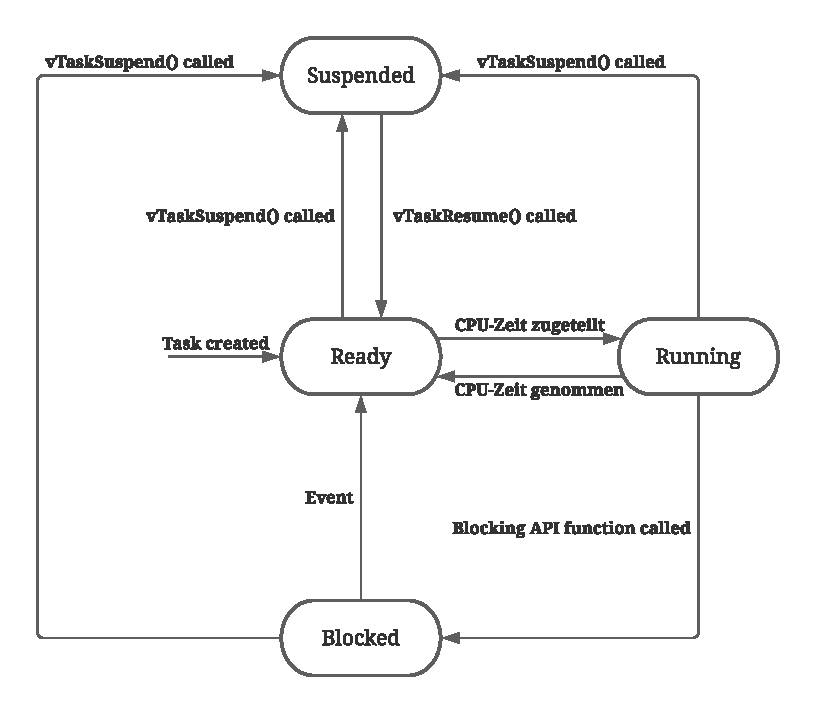
\includegraphics[height=12cm, width=12cm]{./attachments/FreeRTOS_Task_States.pdf}
    \caption{FreeRTOS Task States Quelle: \parencite{freertos-task-states}}
    \label{fig:FreeRTOS_Task_States}
\end{figure}

\subsubsection{Interrupts}
Interrupts werden durch ein Ereignis ausgelöst, \ac{zb} von einem bestimmten Wert eines Timers und führt zur einer Unterbrechung der aktuellen Programmausführung, um in der Regel kurzen, aber zeitlich kritischen, Vorgang abzuarbeiten.
Nach der Unterbrechungsanforderung (\ac{irq}) führt der Prozessor eine Unterbrechungsroutine (\ac{isr}) mit erweiterten Privilegien ausgeführt.
Im Anschluss wird der vorherige Zustand des Prozessors wiederhergestellt und die vorherige Ausführung an der unterbrochenen Stelle fortgesetzt \parencite{wiki:008}.


\subsubsection{\ac{freertos} Sys-Tick}
Der \ac{freertos} Sys-Tick, auch System Tick genannt, ist fundemental für die Taskwechsel in \ac{freertos}, dieser Interrupt wird standartmäßig jede Millisekunde aufgerufen.
Dieser Wert bietet eine gute Balance zwischen Taskgeschwindigkeit und Overhead von Taskwechsel.
Bei jedem Sys-Tick wird die \ac{freertos} Funktion 'vTaskSwitchContext()' aufgerufen, diese überprüft ob eine höher priorisierte Task unblocked, also ausführbar geworden ist und falls dies zutrifft wird ein Taskwechsel auf die höher priorisierte Task durchgeführt.
\end{document}
